% -*- latex -*-
%%%%%%%%%%%%%%%%%%%%%%%%%%%%%%%%%%%%%%%%%%%%%%%%%%%%%%%%%%%%%%%%
%%%%%%%%%%%%%%%%%%%%%%%%%%%%%%%%%%%%%%%%%%%%%%%%%%%%%%%%%%%%%%%%
%%%%
%%%% This text file is part of the source of slides for
%%%% `The Art of HPC, vol 1: The Science of Computing'
%%%% by Victor Eijkhout, copyright 2012
%%%%
%%%%%%%%%%%%%%%%%%%%%%%%%%%%%%%%%%%%%%%%%%%%%%%%%%%%%%%%%%%%%%%%
%%%%%%%%%%%%%%%%%%%%%%%%%%%%%%%%%%%%%%%%%%%%%%%%%%%%%%%%%%%%%%%%

\Level 1 {Latency hiding / communication minimizing}

\begin{frame}
Sparse matrix vector product induces ghost region;

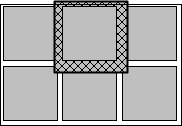
\includegraphics[scale=.5]{ghost}

Is this important?
\begin{itemize}
\item No: surface/volume argument
\item Yes: communication is much slower than computation
\item Case of multiple products is considerably more interesting
\end{itemize}
\end{frame}

\begin{frame}{Optimization of multiple products}
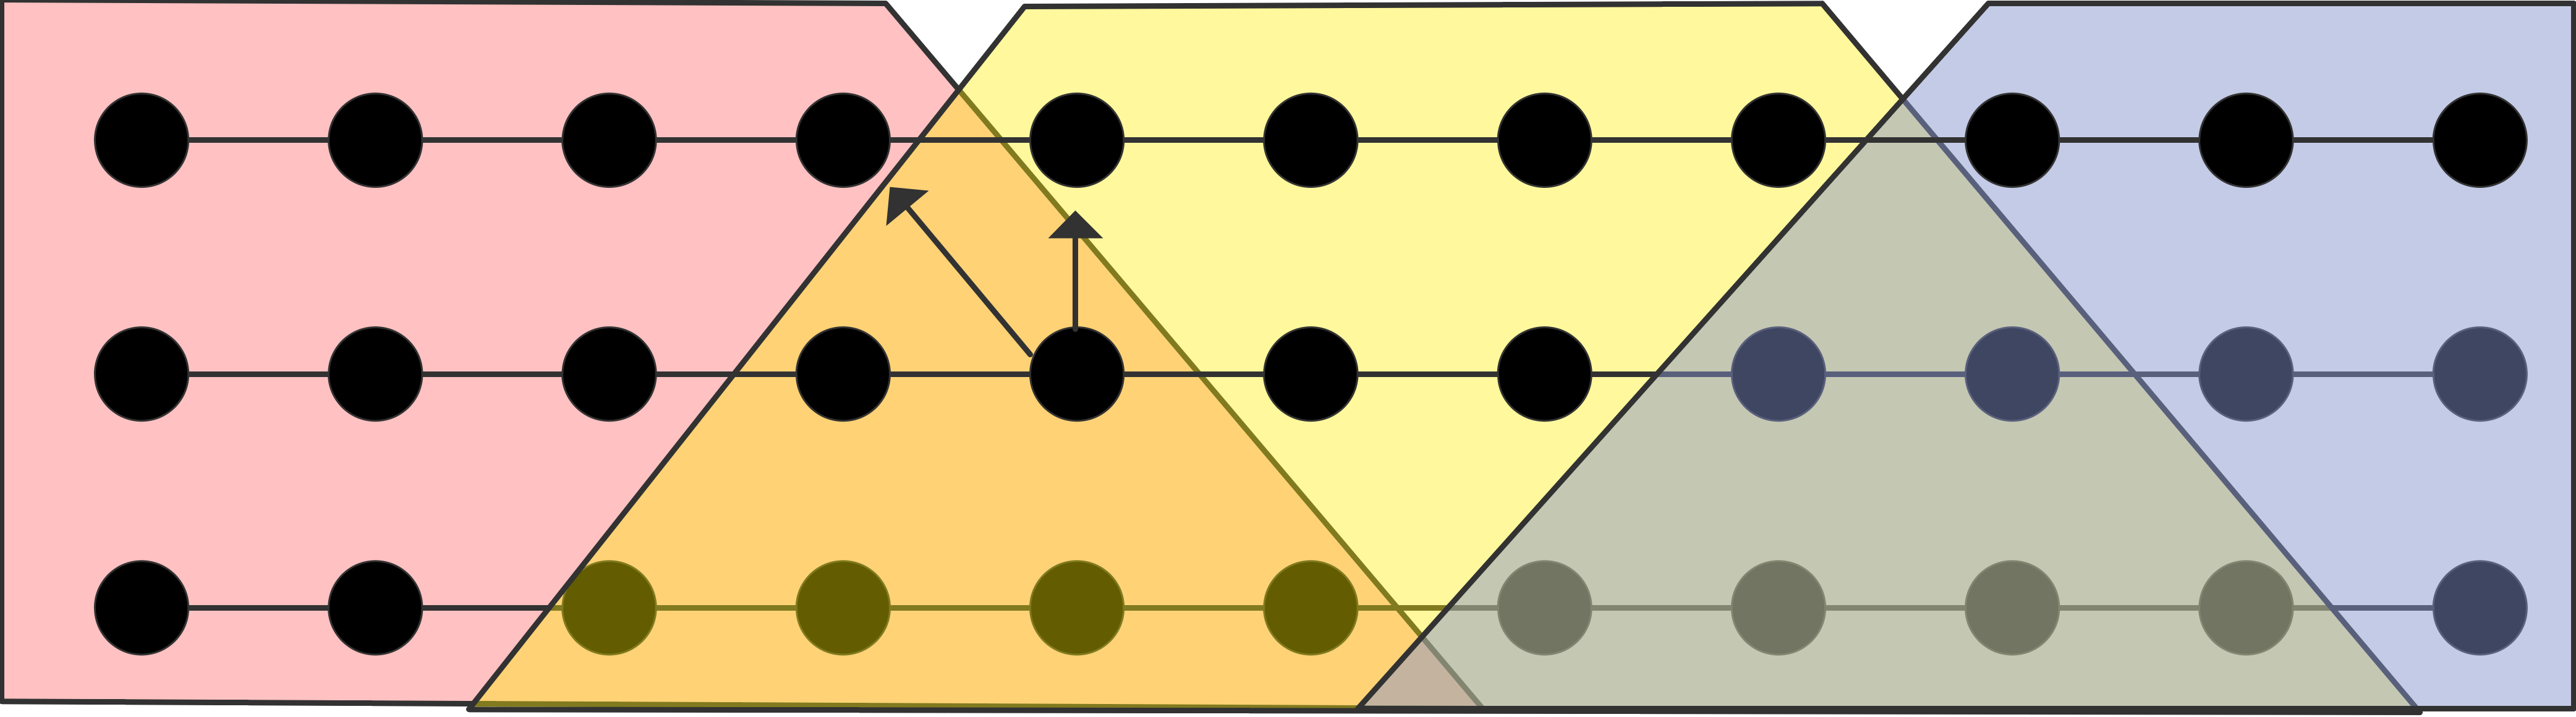
\includegraphics[scale=.07]{grid-update-overlap}

Recursive closure of the halo:
\begin{itemize}
\item Only one latency
\item On-node code can be optimized (caching or cache-oblivious)
\end{itemize}
\end{frame}

\begin{frame}{Latency hiding}
  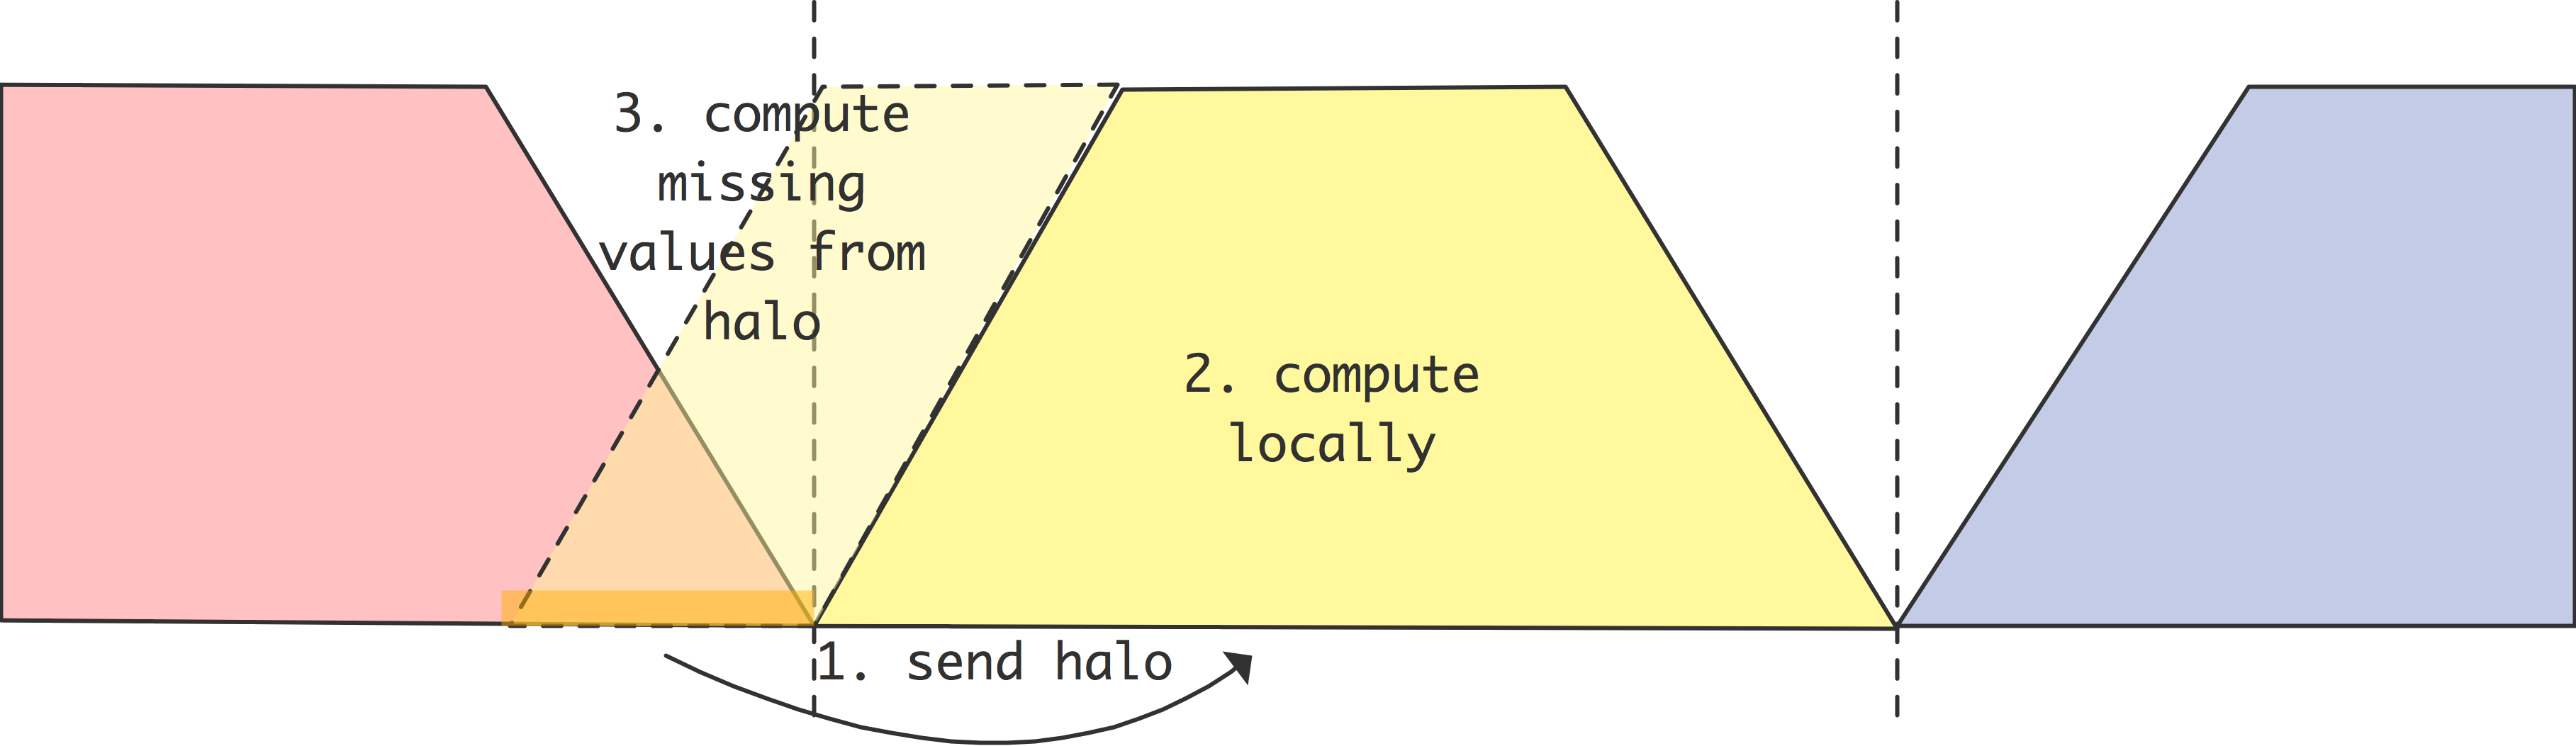
\includegraphics[scale=.08]{grid-update-local}

Overlap halo transfer with local computation:\\
programming complication
\end{frame}

\begin{frame}{Communication minimizing}
Optimal solution (`communication avoiding'):
\begin{itemize}
\item Half the communication
\item half the redundant work
\item Complication: local work done in two stages
\end{itemize}
  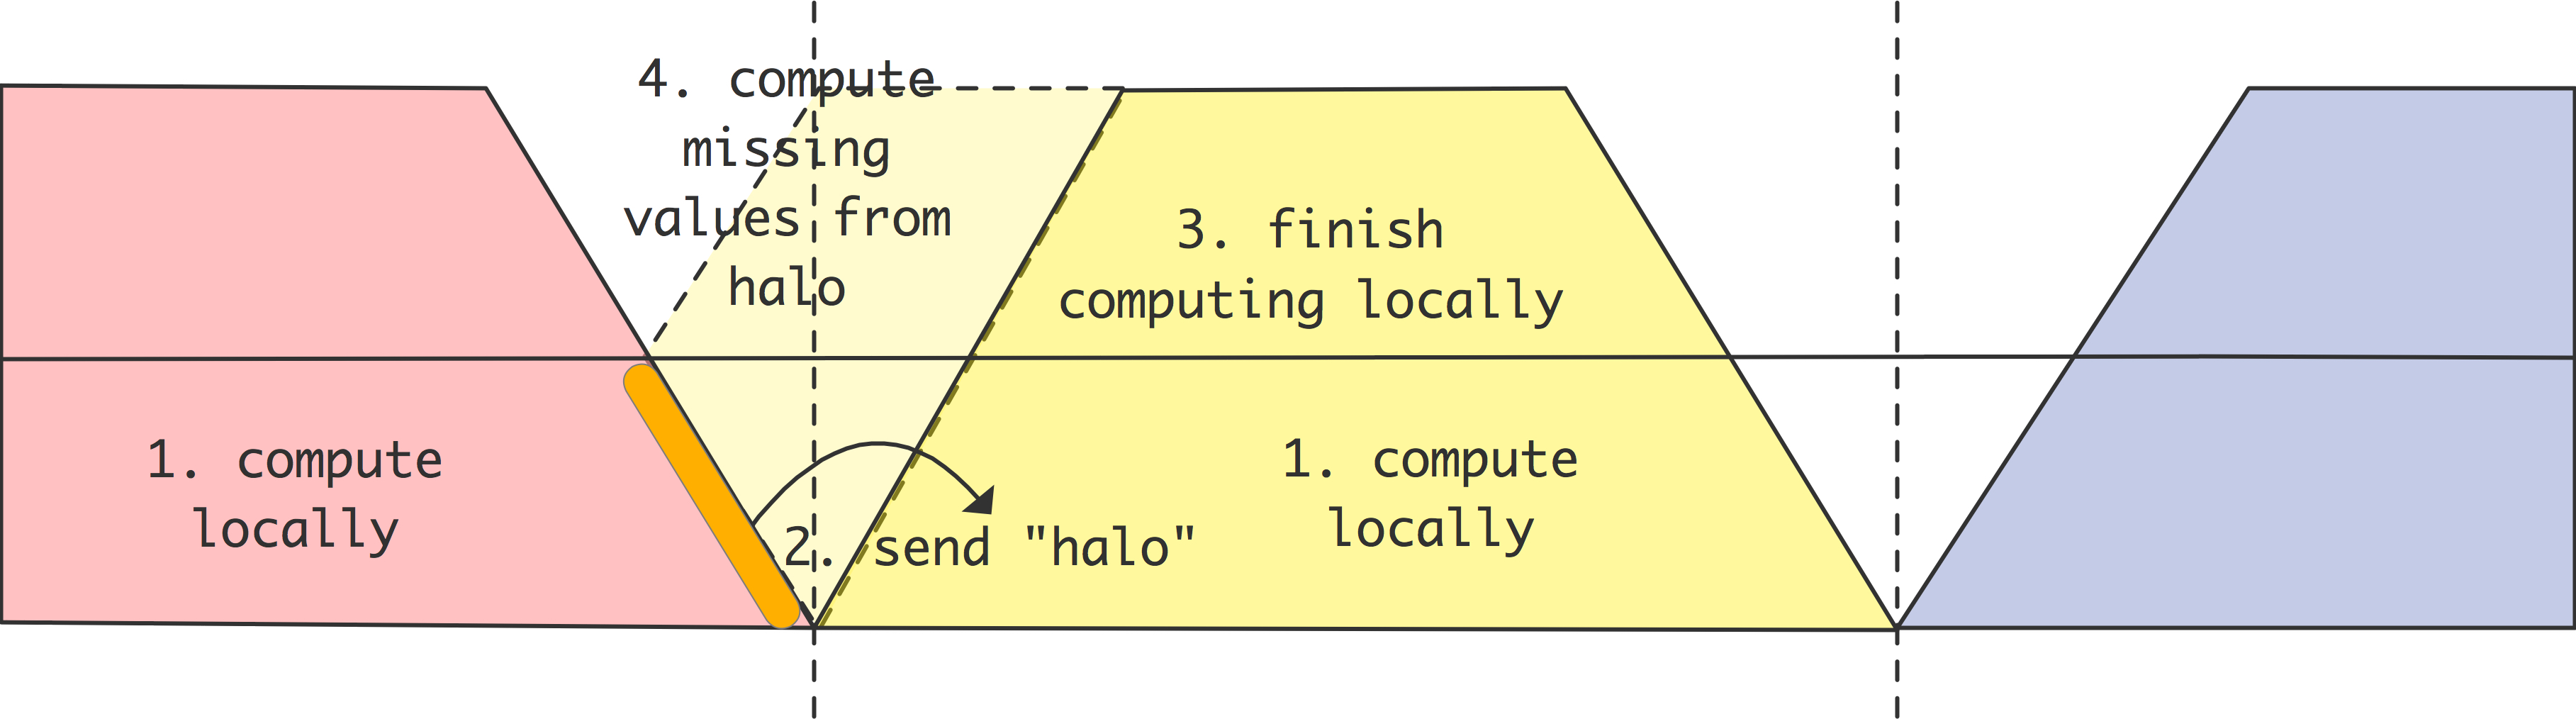
\includegraphics[scale=.08]{grid-update-minimal}
\end{frame}

